\documentclass[a4paper]{article}

\usepackage{INTERSPEECH2018}
\usepackage{amsmath,graphicx}
\usepackage{epsfig,epstopdf,subfigure,slashbox}
\usepackage{amsfonts}
\usepackage{datetime,algorithm,algorithmic,multirow}
\usepackage{xcolor,color}
\usepackage{cite}
\usepackage{amsthm}
\usepackage{array}
\DeclareMathOperator*{\argmax}{argmax}
\pagestyle{empty}

% \tolerance=1000
% \emergencystretch=\maxdimen
% \hyphenpenalty=1000
% \hbadness=1000
\newcommand{\tabincell}[2]{\begin{tabular}{@{}#1@{}}#2\end{tabular}}


% Title.
% ------
%\title{Speech Emotion Recognition Considering Emotion Distribution Information in Dimensional Emotion Space with Emotion-Pair based Framework }
\title{Emotion Recognition from Variable-Length Speech Segments Using Deep Learning on Spectrograms}
% Single address.
% ---------------
\name{Xi Ma$^{1,3}$, Zhiyong Wu$^{1,2,3}$, Jia Jia$^{1,3}$, Mingxing Xu$^{1,3}$, Helen Meng$^{1,2}$, Lianhong Cai$^{1,3}$}

\address{$^1$Tsinghua-CUHK Joint Research Center for Media Sciences, Technologies and Systems,\\
Graduate School at Shenzhen, Tsinghua University, Shenzhen 518055, China\\
  $^2$Department of Systems Engineering and Engineering Management,\\
  The Chinese University of Hong Kong, Shatin, N.T., Hong Kong SAR, China\\
  $^3$Tsinghua National Laboratory for Information Science and Technology (TNList),\\
  Department of Computer Science and Technology, Tsinghua University, Beijing 100084, China}

\email{max15@mails.tsinghua.edu.cn, \{zywu,hmmeng\}@se.cuhk.edu.hk, \{jjia,xumx,clh-dcs\}@tsinghua.edu.cn}
%  {\small \tt max15@mails.tsinghua.edu.cn}, {\small \tt \{zywu,hmmeng\}@se.cuhk.edu.hk}, {\small \tt \{jjia,xumx,clh-dcs\}@tsinghua.edu.cn}}


\linespread{0.94}
\begin{document}

\maketitle
%
\begin{abstract}
In this work, an approach of emotion recognition is proposed for variable-length speech segments by applying deep neutral network to spectrograms directly. The spectrogram carries comprehensive para-lingual information that are useful for emotion recognition. We tried to extract such information from spectrograms and accomplish the emotion recognition task by combining Convolutional Neural Networks (CNNs) with Recurrent Neural Networks (RNNs). To handle the variable-length speech segments, we proposed a specially designed neural network structure that accepts variable-length speech sentences directly as input. Compared to the traditional methods that split the sentence into smaller fixed-length segments, our method can solve the problem of accuracy degradation introduced by the speech segmentation process. We evaluated the emotion recognition model on the IEMOCAP dataset over four emotions. Experimental results demonstrate that the proposed method outperforms the fixed-length neural network on both weighted accuracy (WA) and unweighted accuracy (UA).
\end{abstract}

\noindent\textbf{Index Terms}: Speech Emotion Recognition, Variable-Length Speech Segments, Spectrogram, Deep Neural Network.

\section{Introduction}

Emotion recognition plays an important role in many applications, especially in human-computer interaction systems that are increasingly common today. As one of the main communication media between human beings, voice has attracted wide attentions from researchers~\cite{ayadi2011}. Speech contains a wealth of emotional information. How to extract such information from speech signal is of great importance for automatic speech emotion recognition.

As an important part of speech emotion recognition, the extraction of the most relevant acoustic features has attracted lot of research interests. Most of these researches are devoted to designing some hand-crafted features most distinctive for emotion recognition. Recently, a trend in the machine learning community has emerged towards deriving a representation of the input signal directly from raw, unprocessed data. The reason behind this idea is that the network can learn an intermediate representation of the raw input signal automatically that better suits the task at hand and hence leads to performance improvement. Motivated by this, we tried to construct a emotion recognition system by virtue of a specially designed variable-length deep neural network that can derive the emotion category directly from the spectrogram of the input speech.

A spectrogram is a time-frequency decomposition of a signal that indicates its frequency content over time. In our work, Convolutional Neural Networks (CNNs) are first constructed to learn effectively spatial spectrogram patterns that represent the emotional information; Recurrent Neural Network (RNNs) are then used to model the temporal structure across the sentence being represented by the spectrogram; the final emotion categories are derived by a fully-connected layer.

The idea of this work is similar to Satt's previous work~\cite{satt2017}. However, our neural network possesses the advantage of being able to handle the variable-length speech segments. Compared to splitting the speech input into the smaller and fixed-length segments, our method can solve the loss of accuracy introduced by the speech segmentation process. In the IEMOCAP dataset~\cite{busso2008}, we can achieve a weighted accuracy (WA) of 71.45\% using 5-fold (leave-one-session out) cross validation, which is a 2.65\% absolute (3.85\% relative) improvement over the fixed-length approach. The unweighted accuracy (UA) on the same dataset is 64.22\%, which also outperforms the fixed-length approach with 4.82\% absolute (8.11\% relative) improvement.

The rest of the paper is organized as follows. Section~\ref{sec:related_work} summarizes the previous related work. Comparison between variable-length method and fixed-length method is shown in Section~~\ref{sec:var_len_vs_fixed_len}. The spectrogram extraction and the variable-length neural network structure is then detailed in Section~\ref{sec:implementation_details}. Experiments results are presented in Section~\ref{sec:experiments}. Section~\ref{sec:conclusion} concludes the paper.

\section{Related Work}
\label{sec:related_work}

% As a common issue for speech emotion recognition, feature extraction aims to design functions that map the raw speech signal to the most relevant representation to the emotions. There have been many studies on feature extraction for speech emotion recognition. In~\cite{ma2017, busso2009, cowie2001, vayrynen2013}, prosody-based acoustic features, including pitch-related, energy-related and timing features have been widely used for recognizing speech emotion. Spectral-based acoustic features also play important role in emotion recognition, such as Linear Prediction Coefficients (LPC)~\cite{bellanger1978}, Linear Prediction Cepstral Coefficients (LPCC)~\cite{atal1974} and Mel-frequency Cepstral Coefficients (MFCC)~\cite{davis1980}. In~\cite{gobl2003}, voice quality features have also been shown to be related to emotions.

In the recent years, deep learning methodologies and tools have been introduced to the speech processing area, and used for feature extraction, classification/regression, or both ~\cite{han2014, lee2015, huang2014, le2013, rana2016, chernykh2017}. Researchers have shown that replacing hand-crafted low-level (frame-level) features with statistical learning on the raw signal with different layers of the deep network can significantly enhance the accuracy of classification and regression solutions. In speech recognition, one of the first studies that suggested learning better features for automatic speech recognition (ASR) that used directly the speech waveform was Jaitly and Hinton~\cite{jaitly2012}. Although they did not train the system in an end-to-end manner, they proposed learning an intermediate representation by training a Restricted Boltzmann Machine directly on the speech time signal. Bhargava and Rose~\cite{bhargava2015} used stacked bottleneck deep neural networks (DNNs) trained on windowed speech waveforms and obtained results only slight worse than corresponding MFCC on the same architecture. Sainath et al. match the performance of a large-vocabulary speech recognition (LVCSR) system based on log-Mel filterbank energies by using a Convolutional, LSTM-DNN~\cite{sainath2015a, sainath2015b}. In~\cite{hannun2014, amodei2015}, a recently published state of the art robust speech recognition system is described based on linearly-spaced spectrograms. Besides, direct use of Mel-scale spectrograms for speaker recognition was proved successful as well~\cite{variani2014}.

In the field of speech emotion recognition, several studies have been carried out using deep neural network for feature learning. Recently, George et al.~\cite{trigeorgis2016} proposed a convolutional recurrent neural network that operates on the raw signal, to perform an end-to-end spontaneous emotion prediction task from speech data. Satt et al.~\cite{satt2017} also combined CNN with LSTM to classify emotions from linearly-spaced spectrograms, which achieves beyond the state-of-the-art accuracy on the common benchmarking dataset IEMOACP. However, all of these methods split the speech input into the smaller and fixed-length segments, which introduce a loss of accuracy in the training and predicting stage. Our method proposed to use a variable-length neural network to solve this problem.

\section{Emotion Recognition with Variable-Length Deep Neural Network}
\label{sec:var_len_vs_fixed_len}

\subsection{Problems of Fixed-Length Method}
\label{ssec:problem_fixed_len}

In~\cite{satt2017}, they first split each sentence longer than 3 seconds to shorter sub-sentences of equal length. The part of no longer than 3 second is padded to 3 second with zero after extracting spectrograms. Each sub-sentence is assigned the emotion label of the corresponding whole sentence. These shorter sub-sentences are used throughout the proposed system, for both training and testing stages. During testing phrase, the prediction of the emotion category for the whole sentence is achieved by averaging the posterior probabilities of the respective sub-sentences. Although this method can reduce the difficulty for constructing neural network (ensure that the lengths of inputs are equal), some errors will be introduced. Actually, it is not a good treatment to assign each sub-sentence the emotion label of the corresponding whole sentence. The observation indicates that only a part of voice contains obvious non-neutral emotional information in the non-neutral emotional sentence. In other words, some shorter sub-sentences that belong to a sentence with non-neutral emotion, may not contain any non-neutral emotional information. The use of such sub-sentences for training neutral network may lead to the confusion of the network in identifying the neutral emotion and the non-neutral emotions. However, when we listen to the whole sentence, the neural speech segments can enhance the feeling of emotional speech segments. Hence, it is desirable to design an architecture that can lean such contractive characteristics and recognize emotions using the entire speech sentence.

% To further examine the difference between two speech segments from the same sentence, let's look at spectrograms. The Figure~\ref{fig:spectrogram} below show the spectrograms of two different speech segments (length is 3s), which from the same sentence labeled as Angry.

% \begin{figure}[htb]
%     \begin{minipage}[b]{.42\linewidth}
%     \centering
%     \centerline{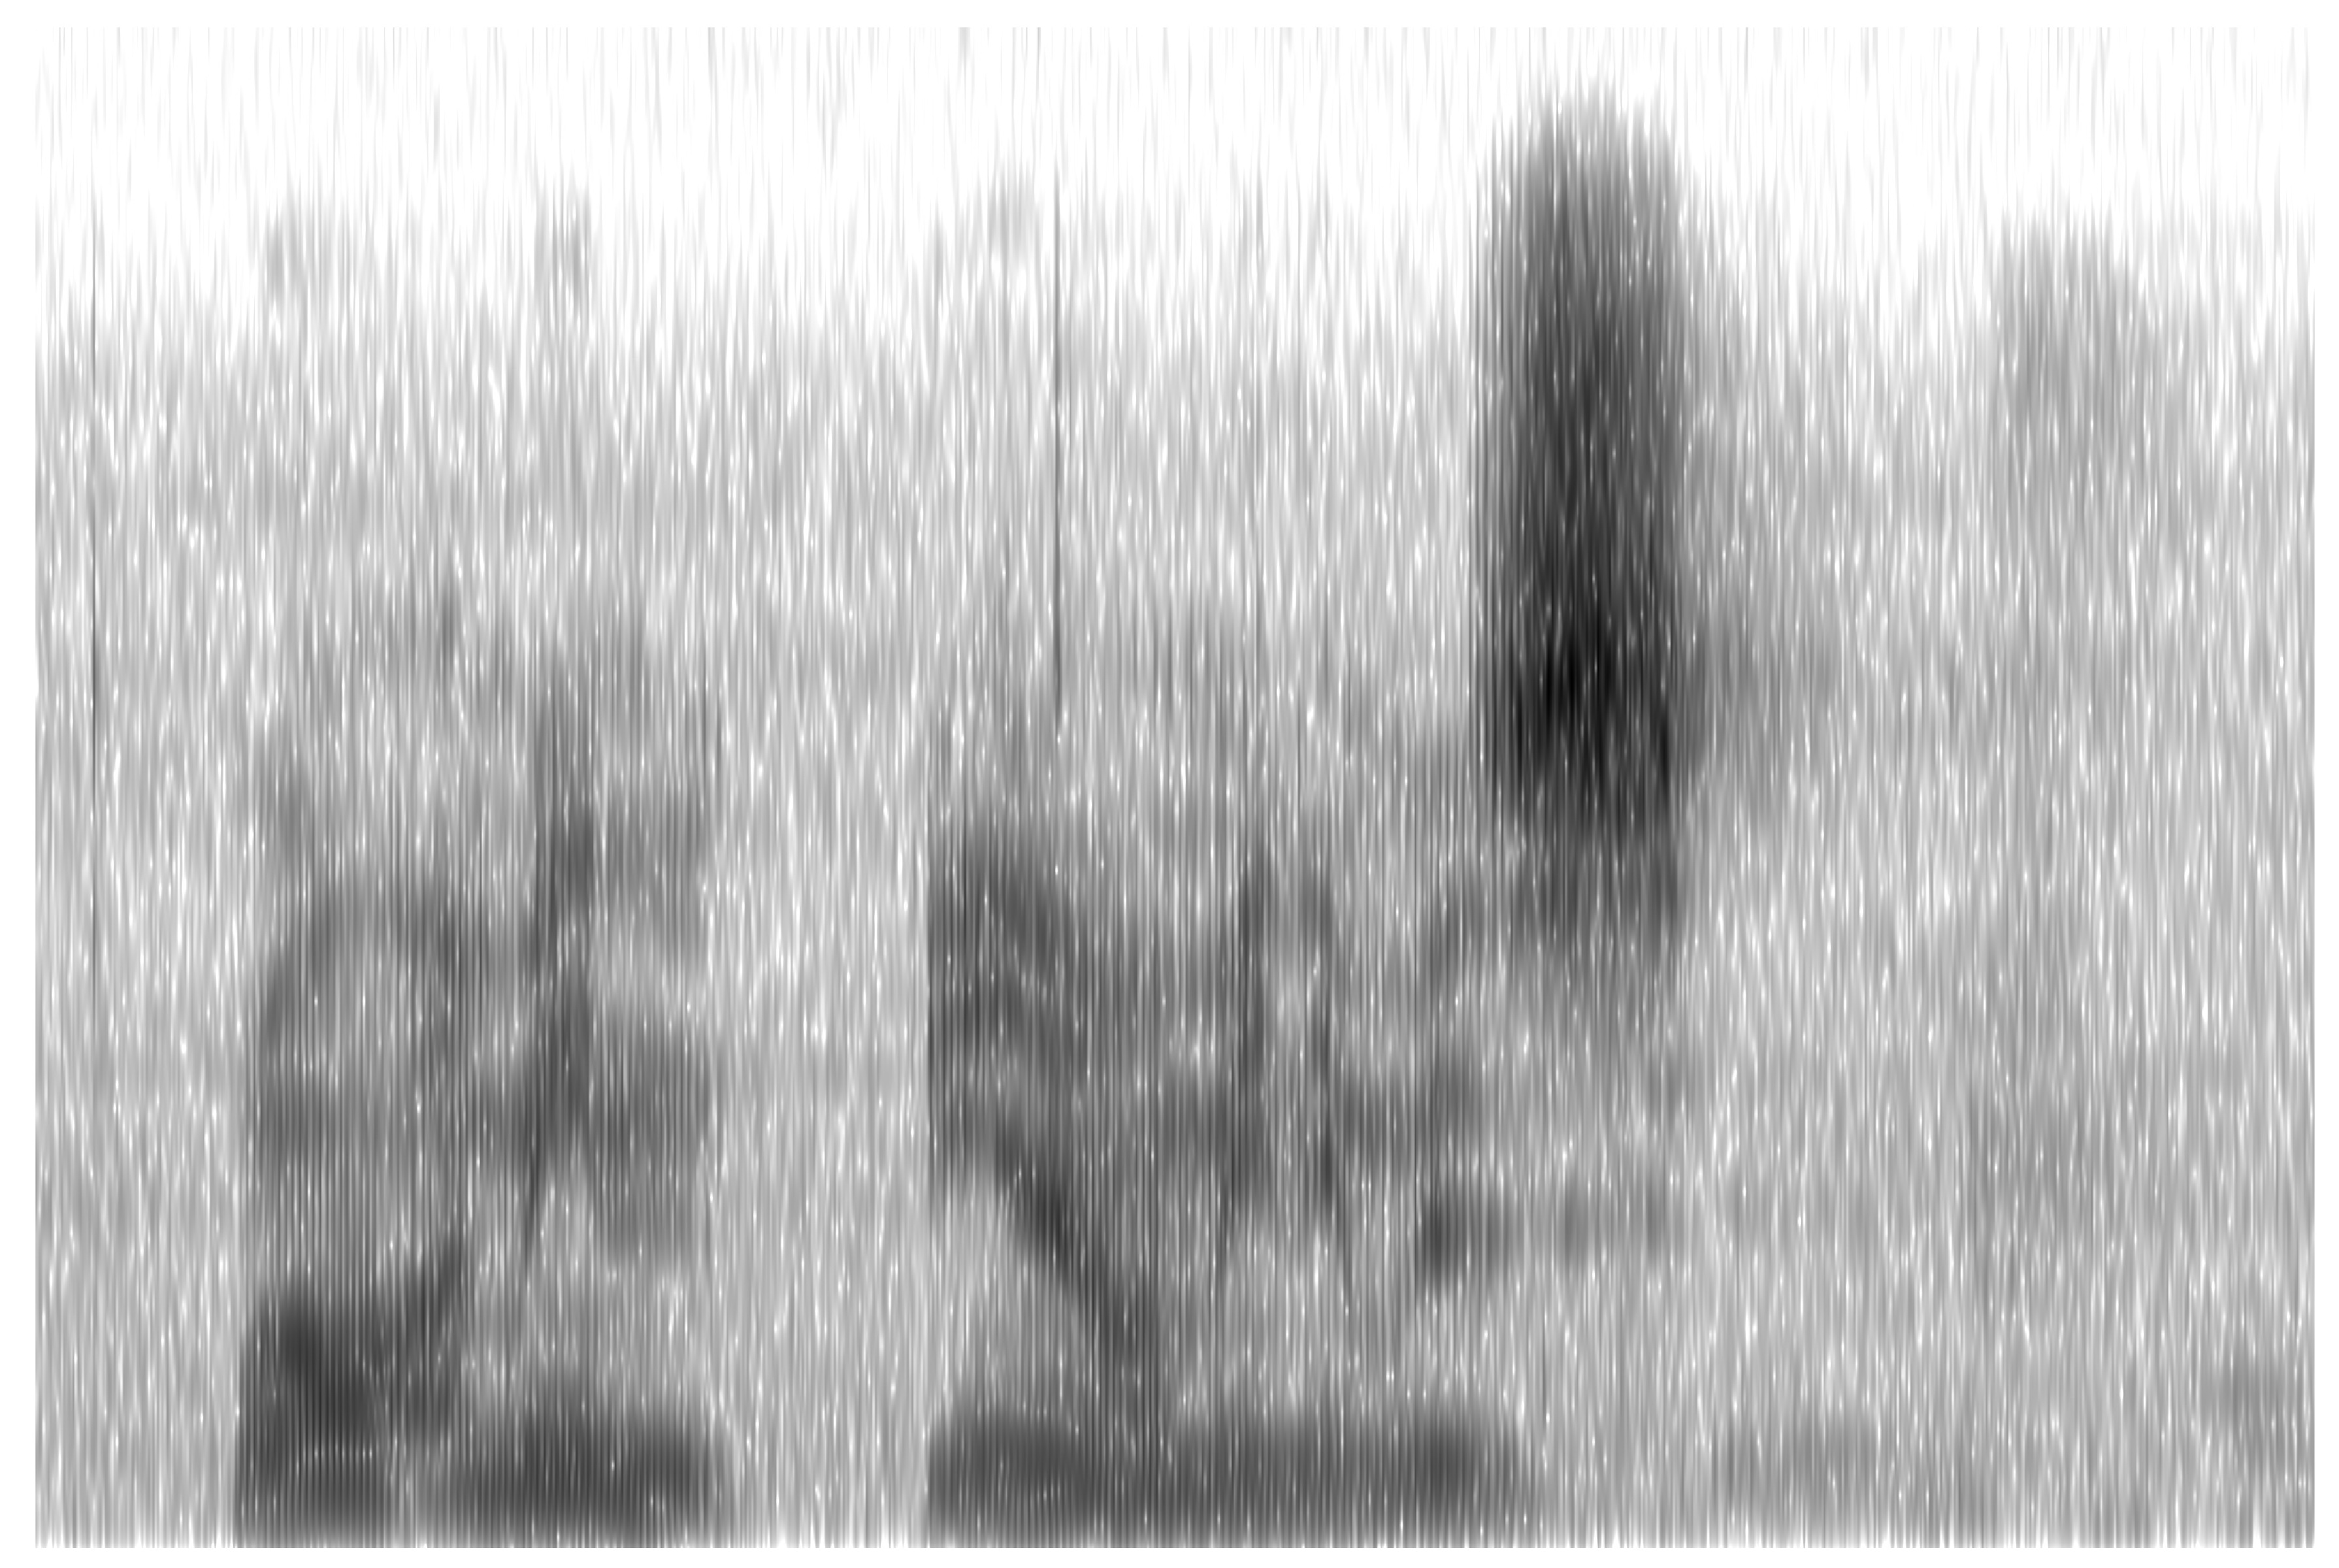
\includegraphics[width=4.2cm]{neu}}
%     %  \vspace{1.5cm}
%     \end{minipage}
%     \hfill
%     \begin{minipage}[b]{0.42\linewidth}
%     \centering
%     \centerline{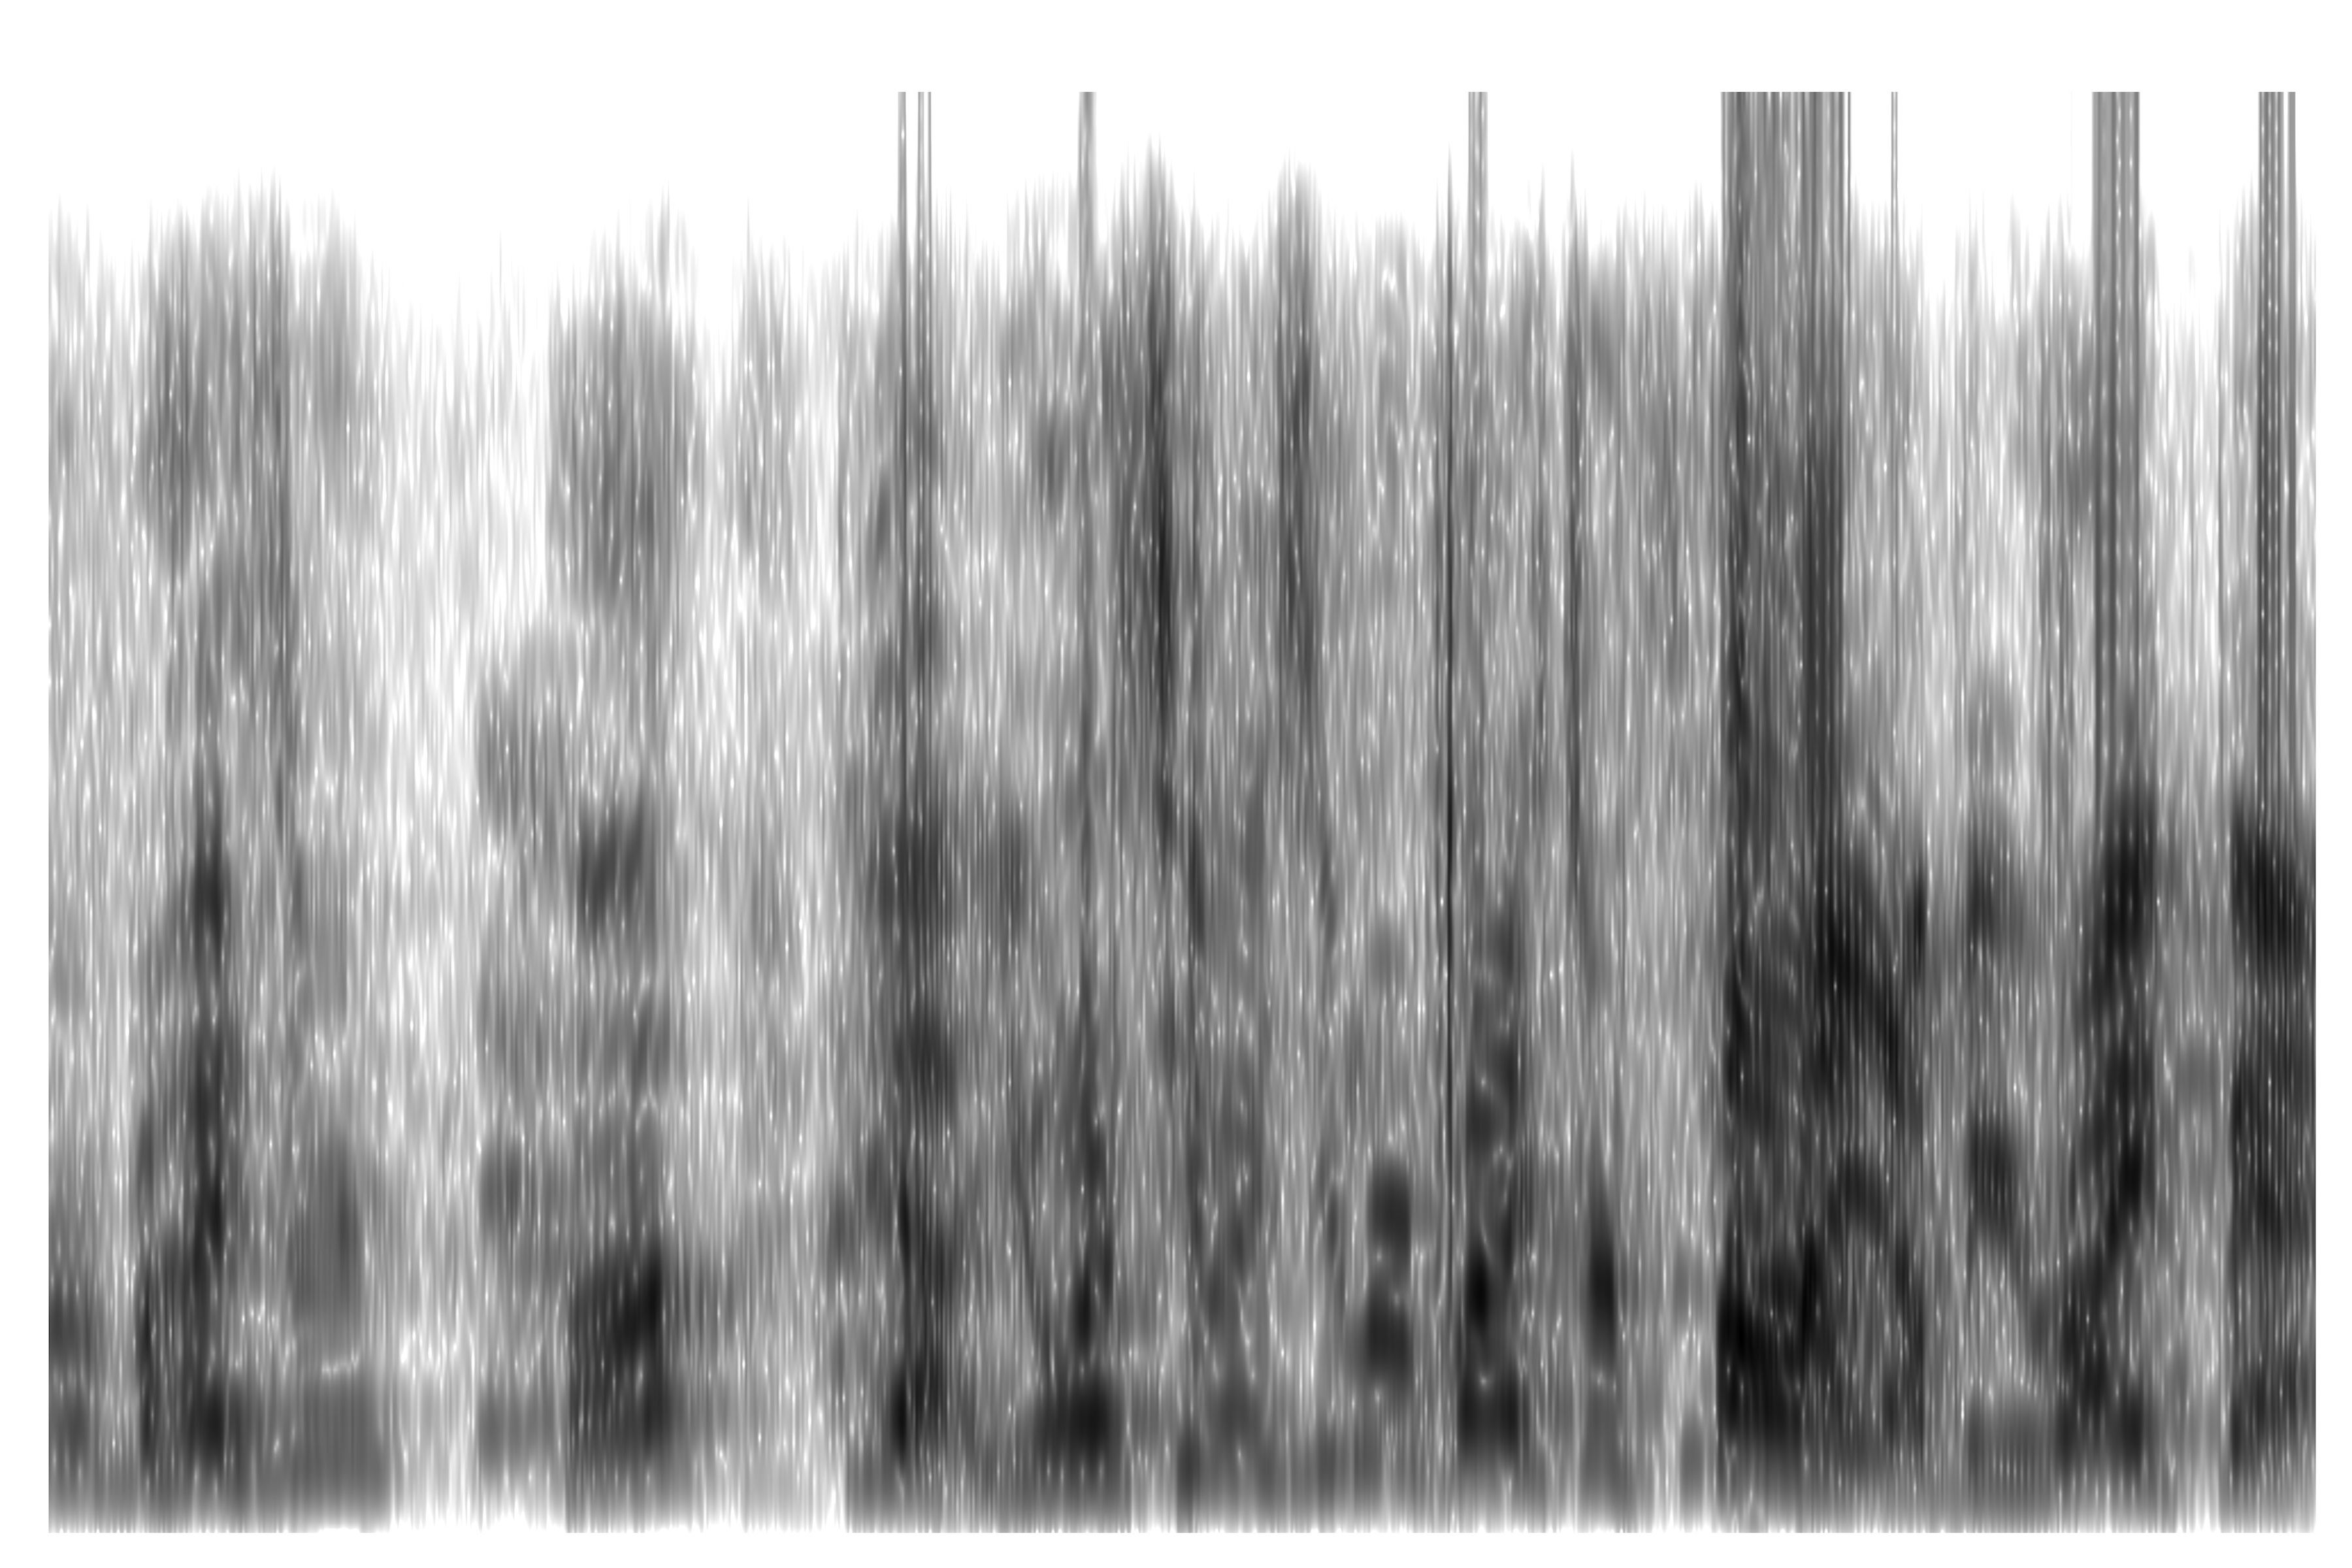
\includegraphics[width=4.2cm]{ang}}
%     %  \vspace{1.5cm}
%     \end{minipage}
%     \setlength{\abovecaptionskip}{0cm}
%     \setlength{\belowcaptionskip}{-0.3cm}
%     \caption{Left: non-emotional spectrogram; Right: emotional spectrogram}
%     \label{fig:spectrogram}
% \end{figure}

% In the Figure~\ref{fig:spectrogram}, the left side $-$ shows the non-emotional spectrogram; the right side $-$ shows the emotional spectrogram. The horizontal axis denotes the time, and the vertical denotes the frequency. The gray scale represents the energy strength $-$ darker colors designate higher energy. It is clearly seen that the right spectrogram shows higher energy than the left spectrogram in most of frequency range. In general, the loudness of angry voice is higher, so the difference of two spectrograms can reflect that the right speech segment looks more like a angry voice than the left speech segment. Besides, through artificial listening, we also find that the right speech segment contains more intense anger, but the left speech segment is more like a neutral speech segment. If all of two speech segments are labeled as Angry, it may cause confusion between Neutral and Angry in the model training and lead to the actual neutral speech segment is misclassified. However, when we listen to the whole sentence, the front neutral speech segment can enhance angry feeling of the back angry speech segment, the so-called angry ending without angry beginning. This problem also occurs in the other non-neutral emotions. 

\subsection{Variable-Length Deep Neutral Network}
\label{ssec:var_len_dnn}

The above problems indicate that using the whole sentence as the input is more reasonable than splitting into several segments. But the lengths of sentences are different in general, so our study aims to design a neural network to handle the variable-length input sequence. 

As we all known, convolutional neural networks (CNNs) can be thought of as a kind of neural network that uses many identical copies of the same neuron. This allows the network to have lots of neurons and express computationally large models while keeping the number of actual parameters $-$ the values describing how neurons behave $-$ that need to be learned fairly small. The commonly used means, especially in computer vision, is to process the inputs of the same size. This is convenient to connect other neural network, such as full connected layer. But in fact, the convolutional neural network just need to train convolutional kernels, so it can also be trained, even if the input size is different.

Recurrent Neural Networks (RNNs) are popular models that have shown great promise in many sequence modeling tasks. They perform the same task for every element of a sequence, with the output being depended on the previous computations. For the computing efficiency, the input sequence is usually fixed-length. The variable-length sequence is usually padded into the same length. But we can ignore the outputs of invalid padding time-steps, so that the variable-length sequence can be processed correctly.

We hypothesized that the convolutional neural networks, capable of learning spatial patterns, will learn effectively spatial spectrogram patterns that represent the emotional information. We also hypothesized that adding an recurrent neural network layer will help learning the temporal behavior across the sentence. These two types of neural networks will be used to process the variable-length input sequence. The implementation details are presented in the next section.  

\section{Implementation Details}
\label{sec:implementation_details}

The input of the variable-length deep neutral network is the spectrogram of the whole sentence, and the output is the classification result of emotion category for the sentence. For comparison, we use the similar spectrogram extraction setting and neural network as those used in~\cite{satt2017}.

\subsection{Spectrogram Extraction}
\label{ssec:spectrogram_extraction}

% \begin{figure}[!htb]
% %\setlength{\abovecaptionskip}{-0.3cm}
% %\setlength{\belowcaptionskip}{-0.5cm}
% \centering
% \centerline{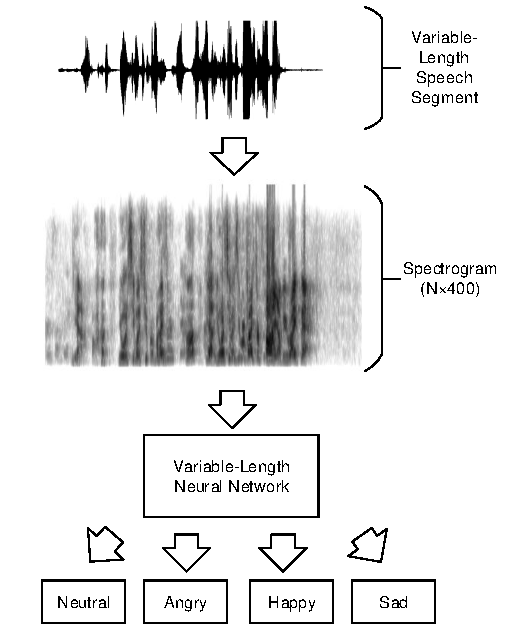
\includegraphics{flow}}
% %  \vspace{2.0cm}
% \caption{Flow chart of our emotion recognition system.}
% \label{fig:flow}
% \end{figure}

% \subsection{Spectrogram Extraction}
% \label{ssec:spectrogram_extraction}

The speech signal in the IEMOCAP dataset is sampled at 16KHz and organized as single sentences with duration from less than a second to about 20 second. Each sentence is labeled with one emotion. A sequence of overlapping Hamming windows is applied, with frame step (window shift) of 10msec, and frame length (window size) of 40 msec. For each frame we calculate a DFT of length 1600 (for 10Hz grid resolution). We use the frequency range of 0-4KHz, ignoring the rest. Following aggregation of the short-time spectra, we obtain a matrix of size NxM, where N is variable for different sentences, representing the selected timing grid resolution,  and M=400 is equal to the selected frequency grid resolution. The DFT data is then converted to log power spectrum, and then normalized with z normalization using the mean and standard deviation of the training dataset.

To improve the computing efficiency, the speech samples are ordered by the sentence lengths; and the spectrograms with similar timing lengths are organized into the same batch and padded with zero to the max length of the spectrogram in the current batch.  Parallel computing can then be achieved for a batch of samples during training stage.

\subsection{Deep Neural Network}
\label{ssec:deep_neural_network}

In our work, the input sequence are padded into the same length with zero in the same batch during training stage, but the length between different batches are different. And no padding is used during predicting stage. So our neural network needs to possess the capacity to avoid the interference of padding value on the output.  Let $S=[x_1, x_2, ..., x_V, ..., x_T]$ be a input sequence, where $S1=[x_1, x_2, ..., x_V]$ is the valid part and $S2=[x_{V+1}, x_{V+2}, ..., x_T]$ is the padding part.

First, for the convolution neutral network, we can use masking to reserve the outputs from $S1$ and ignore the outputs from $S2$, which can be represented as follows:
\begin{equation}
\label{eq:masking}
S_{conv}=Conv(S) \bullet Mask(S)
\end{equation}
where $Conv(S)$ is the output of convolution layer for $S$, $Mask(S)$ is a masking matrix, and $S_{conv}=[y_1, y_2, ..., y_V, ..., y_T]$ is the output sequence with the same length as $S$. The values of the masking matrix are ones for the valid part, and zeros for the padding part. The valid output can be achieved by element-wise multiplication between $Conv(S)$ and $Mask(S)$. Besides, convolutional layers are often interweaved with pooling layers. We need to take care of the border value between the valid part and the padding part, which could introduce the invalid information. For example, let us assume $S_{conv}$ is the input of the max-pooling layer. If the pooling kernel size is 2 and the input path contains $y_V$ and $y_{V+1}$, the output will be $y_{V+1}$ when $y_V<0$ and $y_{V+1}=0$. But the expected value should be $y_V$ because $y_{V+1}$ is a padding value. In our experiment, this problem will lead to the problem that the neural network does not converge. Hence, the $y_V$ will be masked as zero before inputting to the max-pooling layer in our design. In this way, padding or no padding, the same input will produce the same output after convolution layer and pooling layer. It ensures the consistency in training stage and predicting stage, because there is no padding in the predicting stage.

Second, for the recurrent neural network, because speech emotion recognition is a sequence classification problem, we just need the output in the last valid time-step. Assuming $S$ is the input of recurrent neural network, the expected result should be the output at $t=V$. Besides, in the bi-directional recurrent neural network, the output of backward recurrent neural network should be at $t=0$. The final output is the concatenation of the outputs in forward and backward recurrent neural network.

Dozens of combinations of topologies were tested. The best deep neural network topology is depicted in Figure~\ref{fig:network}.

\begin{figure}[!htb]
    \centering
    \centerline{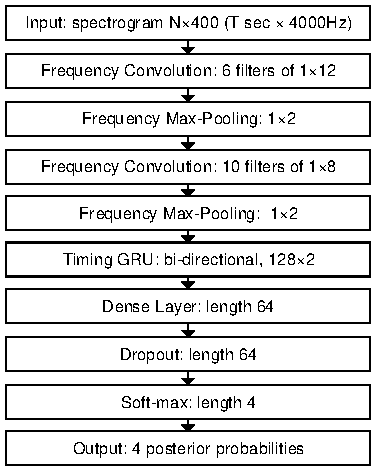
\includegraphics{network}}
    % \setlength{\abovecaptionskip}{0cm}
    % \setlength{\belowcaptionskip}{0cm}
    \caption{Deep neutral network topology}
    \label{fig:network}
\end{figure}

Since the length of sentence is different, we will assign different weights to the loss, in inverse proportion to the length. This ensures that the length of sentence doesn't affect the bias of model. Besides, the IEMOCAP corpus is significantly unbalanced, the number of some emotional categories is obviously more than other emotional categories. The weight, in inverse proportion to the class size, will also be assigned to the loss.

\section{Experiments}
\label{sec:experiments}

\subsection{Experimental Setup}
\label{ssec:experimental setup}

In this work, the IEMOCAP dataset~\cite{busso2008} is used for conducting the experiments. The dataset was designed for studying multimodal expressive dyadic interactions. It was collected using motion capture and audio/video recording (approximately a total of 12h) over 5 dyadic sessions with 10 subjects. Each session consists of a different dyad where one male and one female actor perform scripted plays and engage in spontaneous improvised dialogs elicited through affective scenario prompts. At least three evaluators annotated each utterance in the dataset with the categorical emotion labels chosen from the set: happy, sad, neutral, angry, surprised, exited, frustration, disgust, fear and other. We consider only the utterances with majority agreement (at least two out of three evaluators gave the same emotion label) over the emotion classes of: Angry, Happy, Sad and Neutral. The dataset contains scripted and improvised dialogs. As the script text exhibits strong correlation with the labeled emotions, it may give rise to linguistic content learning, at least partially, which is an undesired side effect. Therefore we used the improvised data only. Such configuration is the same as~\cite{satt2017}, which makes the experimental results comparable between our work and~\cite{satt2017}. The 5-folds cross-validation method is used to conduct the experiments. In each fold, the data from four sessions is used for training the deep neural network, and the data from the remaining session is split $-$ one speaker for validation and the other for the accuracy testing.

The experimental results can be divided into two parts. In the first part, we compare the performance of the variable-length neural network and the fixed-length neural network. In the second part, we show the activations of the recurrent neural network from the variable-length neural network and the fixed-length neural network, whose difference can be used to verify our assumption that the fixed-length method may lead to the confusion of model training. 

\subsection{Experimental Results}
\label{ssec:experimental_results}
First, we conduct emotion recognition experiments by reporting the weighed accuracies (WA) and the unweighted accuracy (UA) of different methods, where WA is the accuracy of all samples in the test set and UA is the average value of the accuracy values of all emotions. Both metrics are standard measurements used in several previous emotion recognition challenge and is adopted in~\cite{satt2017}. Also, owing to the topology of our network is different from \cite{satt2017}, we implement the fixed-length method by using the fixed-length speech segments as the input to our network. This is to ensure that the improvement of performance don't come from topology changing.

In Table~\ref{tab:accuracy_en}, we present weighted accuracy (WA) and unweighted accuracy (UA) in the IEMOCAP dataset, where ``Baseline'' represents the result reported in~\cite{satt2017}, ``Fixed-Length'' represents the fixed-length inputs for our neural network, ``Variable-Length'' represents the variable-length inputs for our neural network. As can be seen, the WA of ``Variable-Length'' is 71.45\%, which is a 2.65\% absolute (3.85\% relative) improvement over ``Baseline''; And the UA also reaches 64.22\%, which is a 4.82\% absolute (8.11\% relative) improvement compared to ``Baseline''. Besides, the WA and UA of ``Fixed-Length'' is also lower than ``Variable-Length'', so this proves that the improvement of performance don't come from parameters changing.

To further analyze the experimental result, we present the confusion matrices of both the fixed-length input and the variable-length input for our network in Table~\ref{tab:cm_const} and Table~\ref{tab:cm_var}. We can find that the recognition accuracies of Neutral for our variable-length network are improved. As we have made the analysis for Section~\ref{ssec:problem_fixed_len}, this is because the confusion between Neutral and other emotions can be alleviated by inputting the whole sentence to the network. Besides, the accuracy of Happy is improved significantly. This is caused by the neutral speech segment in the Happy sentence may be misclassified to other emotions, because these neutral speech segments are very similar by using fixed-length model. Meanwhile, the accuracy of Sad is decreased. It may be that the increasing recall of other non-neutral emotions lead to the decreasing recall of Sad. These results indicate that the variable-length neural network really provides improvement in the recognition accuracy of some emotions.

\begin{table}[htb]
    \setlength{\abovecaptionskip}{0cm}
    \setlength{\belowcaptionskip}{-0.3cm}
    \caption{Comparison of weighted accuracy (WA) and unweighted accuracy (UA) on IEMOCAP dataset}
    \scalebox{0.95}{
    \begin{tabular}{p{3cm}<{\centering} | p{2cm}<{\centering} | p{2cm}<{\centering}}
        \hline
        & WA & UA \\
        \hline
        Baseline & 68.8\% & 59.4\% \\
        \hline
        Fixed-Length & 68.86\% & 57.45\% \\
        \hline
        Variable-Length & 71.45\% & 64.22\% \\
        \hline
    \end{tabular}}
    \label{tab:accuracy_en}
\end{table}

\begin{table}[htb]
    \setlength{\abovecaptionskip}{0cm}
    \setlength{\belowcaptionskip}{-0.3cm}
    \caption{Confusion matrix by using the fixed-length neural network}
    \scalebox{0.9}{
    \begin{tabular}{c|c|c|c|c}
        \hline
            \backslashbox{Actual}{Predict} & Neutral & Angry & Happy & Sad \\
        \hline
            Neutral & \textbf{71.75\%} & 8.88\% & 5.93\% & 13.45\% \\
        \hline
            Angry & 30.84\% & \textbf{58.79\%} & 7.05\% & 3.34\% \\
        \hline
            Happy & 55.92\% & 31.42\% & \textbf{11.72\%} & 0.95\% \\
        \hline
            Sad & 11.41\% & 0\% & 1.02\% & \textbf{87.57\%} \\
        \hline
    \end{tabular}}
    \footnotesize
    \label{tab:cm_const}
\end{table}

\begin{table}[htb]
    \setlength{\abovecaptionskip}{0cm}
    \setlength{\belowcaptionskip}{-0.3cm}
    \caption{Confusion matrix by using the variable-length neural network}
    \scalebox{0.9}{
    \begin{tabular}{c|c|c|c|c}
        \hline
            \backslashbox{Actual}{Predict} & Neutral & Angry & Happy & Sad \\
        \hline
            Neutral & \textbf{73.64\%} & 2.74\% & 12.41\% & 11.21\% \\
        \hline
            Angry & 11.44\% & \textbf{59.55\%} & 26.52\% & 2.5\% \\
        \hline
            Happy & 45.2\% & 13.81\% & \textbf{40.05\%} & 0.95\% \\
        \hline
            Sad & 15.89\% & 0\% & 0.48\% & \textbf{83.64\%} \\
        \hline
    \end{tabular}}
    \footnotesize
    \label{tab:cm_var}
\end{table}

\subsection{Analysis of Network Activations}
\label{ssec:analysis_activation}

It is informative to examine what the deep network learns by looking at the activations. Figure~\ref{fig:rnn_comp} shows the activations of different nodes of recurrent neural network, from a speech sentence labeled as Neutral. The left one shows the activations of the fixed-length model; the right one shows the activations of the variable-length model. The horizontal axis denotes the time, and the vertical denotes the activations of different nodes at recurrent neural network. The gray scale represents the degree of activation $-$ darker colors designate higher activation. We can find that the right stripes are clearer than the left stripes in the activation map. Besides, we also find that the specific emotion has higher activation in specific nodes. Figure~\ref{fig:rnn_emo} shows that the activation maps of recurrent network in three different emotions. The nodes in the red box represents the high degree of activation. As can be observed, the active nodes are similar for Angry and Happy. It is generally known that these two emotions have similar acoustic expressions~\cite{ma2017}. But the active nodes of Sad are obviously different from Happy and Angry. However, owing to the unstable acoustic expression, such specific active nodes cannot be observed in the neutral speech (right of Figure~\ref{fig:rnn_comp}). All these results indicate that there are clear differences between different emotions (including neutral) for the active nodes of the variable-length neural network.  On the other hand, for the fixed-length method, it is hard to observe such trend due to the fuzzy stripes in the activation map (left of Figure~\ref{fig:rnn_comp}). This proves that variable-length method can relieve the confusion between neutral and non-neutral emotions in the fixed-length method.

\begin{figure}[htb]
    \begin{minipage}[b]{0.42\linewidth}
      \centering
      \centerline{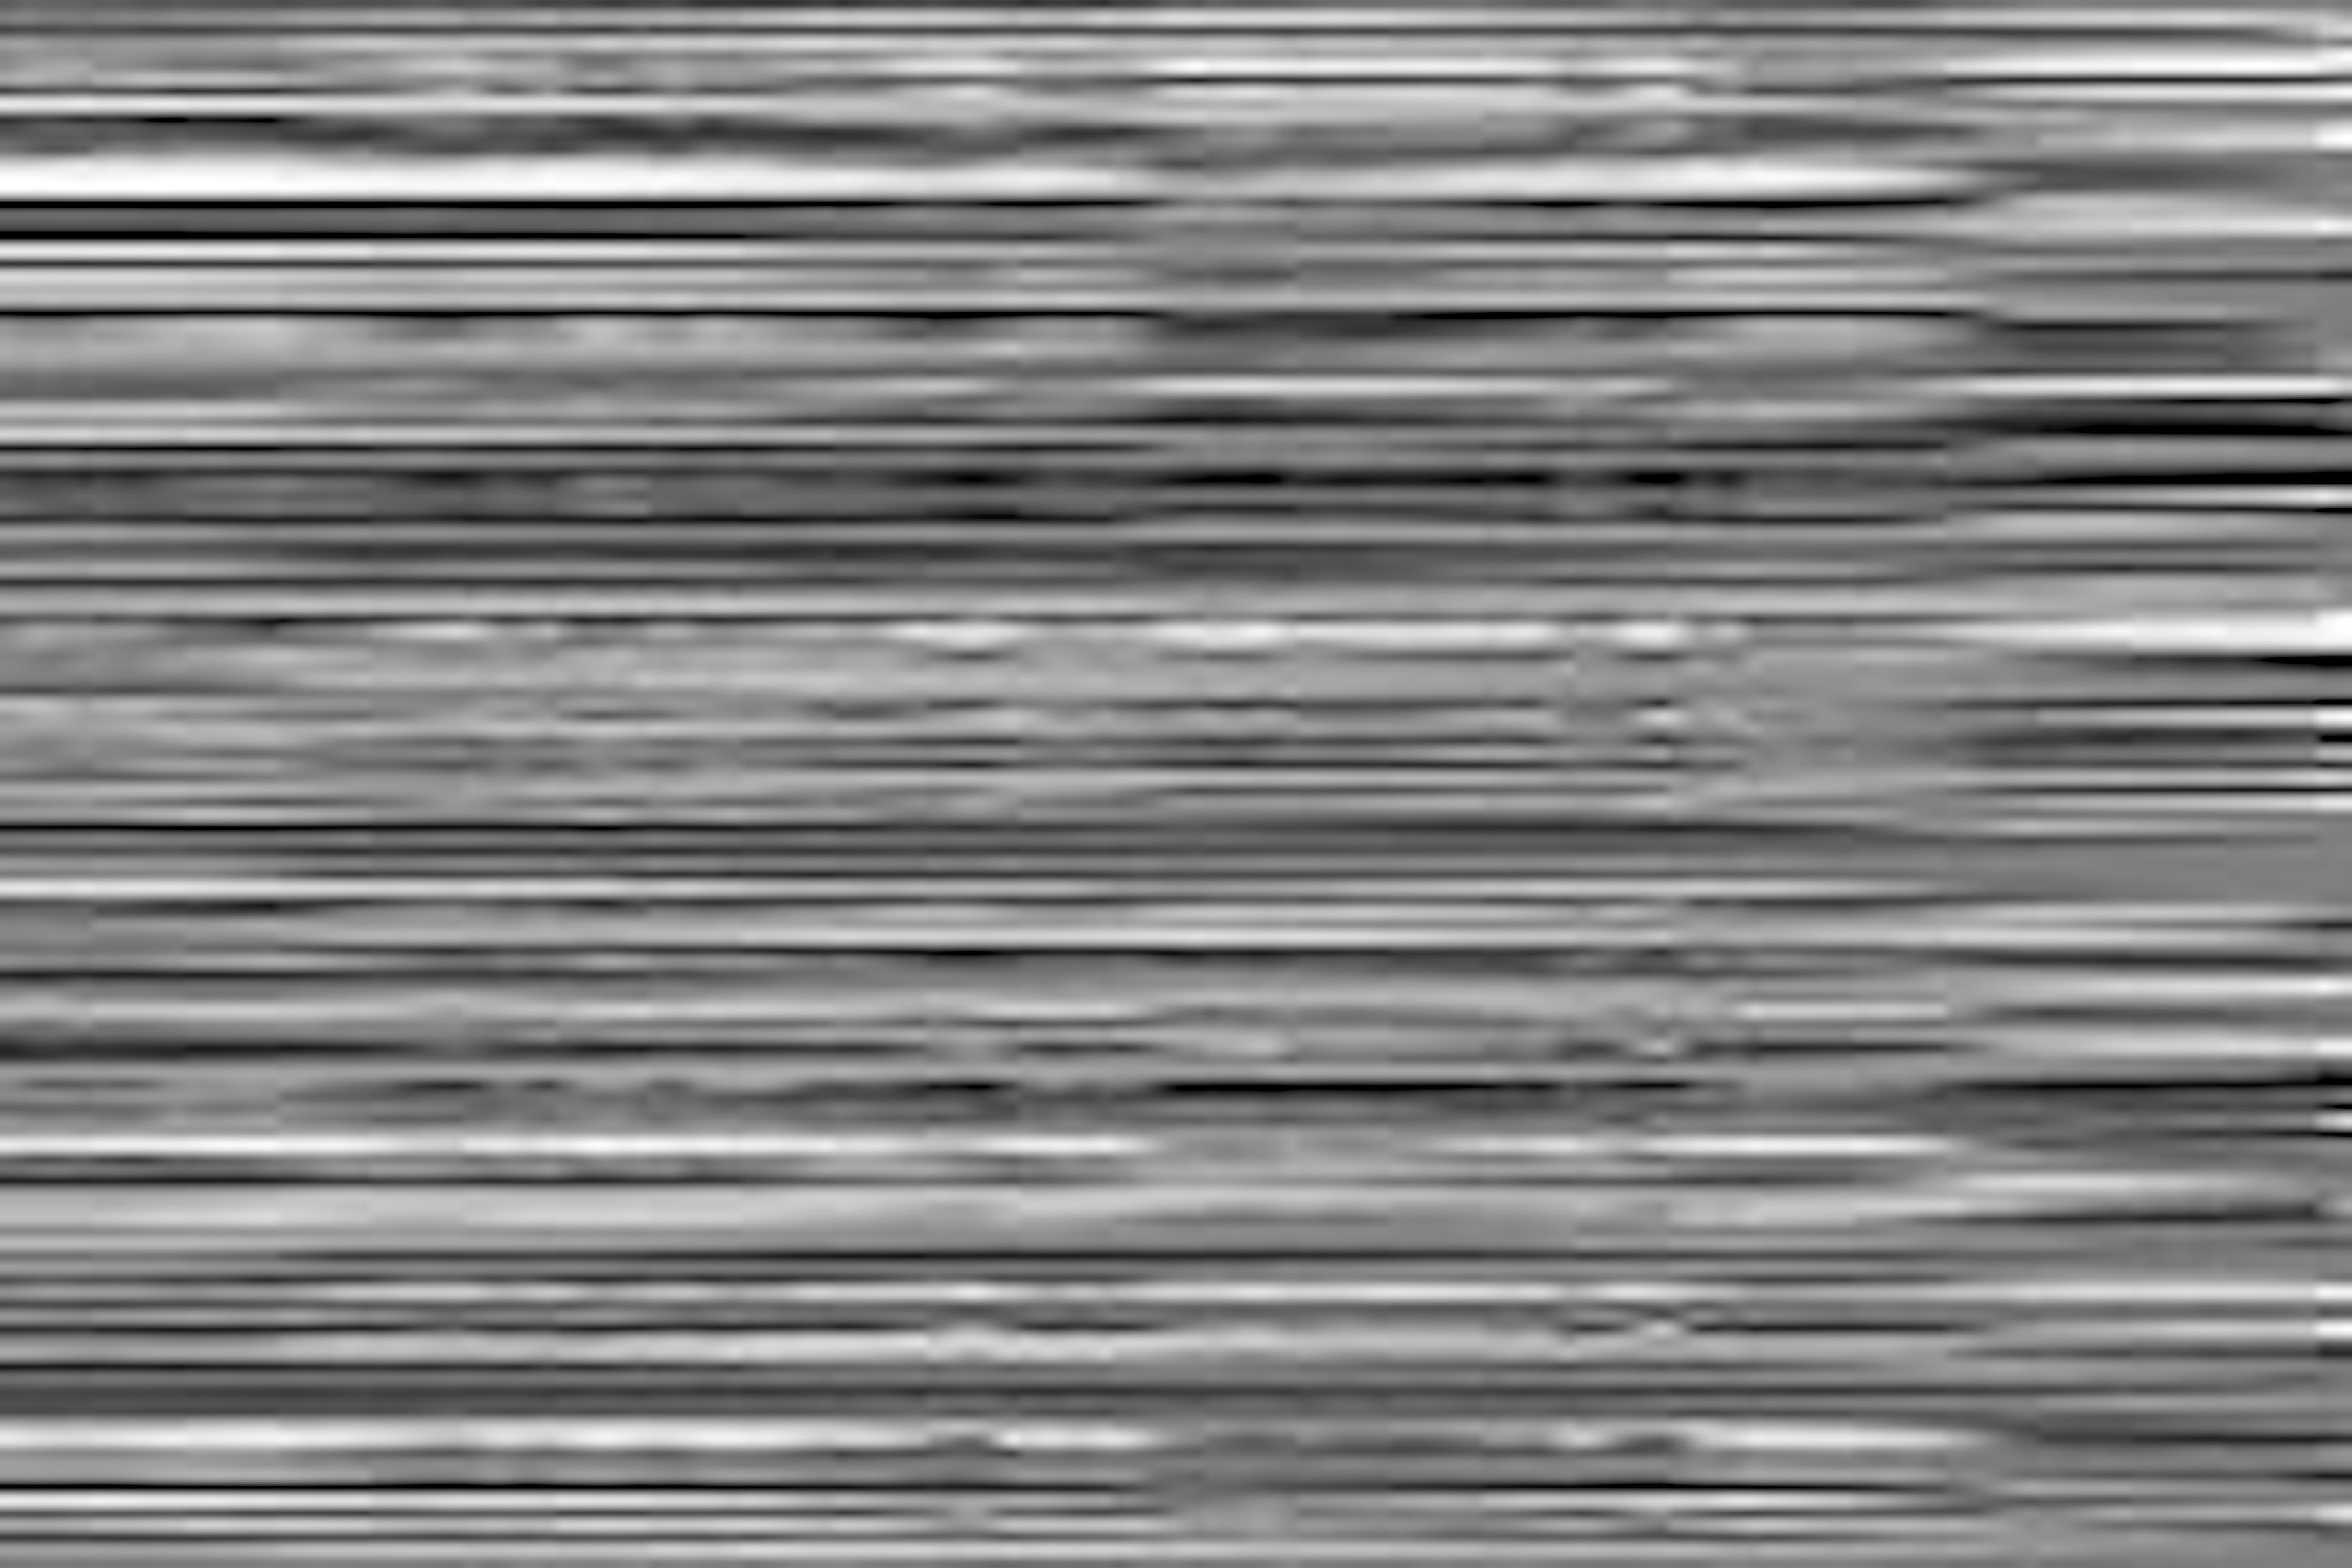
\includegraphics[width=4.2cm]{rnn_out_const_neu_comp}}
    %  \vspace{1.5cm}
    \end{minipage}
    \hfill
    \begin{minipage}[b]{0.42\linewidth}
      \centering
      \centerline{
\includegraphics[width=4.2cm]{rnn_out_var_neu_comp}}
    %  \vspace{1.5cm}
    \end{minipage}
    %
    % \setlength{\abovecaptionskip}{0cm}
    % \setlength{\belowcaptionskip}{0cm}
    \caption{Activations of different nodes for a neutral sentence (Left: Fixed-length; Right: Variable-Length)}
    \label{fig:rnn_comp}
\end{figure}

\begin{figure}[htb]
    \begin{minipage}[b]{0.27\linewidth}
      \centering
      \centerline{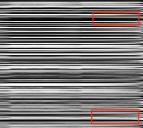
\includegraphics[width=2.7cm]{rnn_out_var_ang}}
    %  \vspace{1.5cm}
    \end{minipage}
    \hfill
    \begin{minipage}[b]{0.27\linewidth}
      \centering
      \centerline{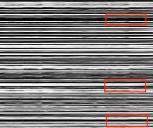
\includegraphics[width=2.7cm]{rnn_out_var_hap}}
    %  \vspace{1.5cm}
    \end{minipage}
    \hfill
    \begin{minipage}[b]{0.27\linewidth}
      \centering
      \centerline{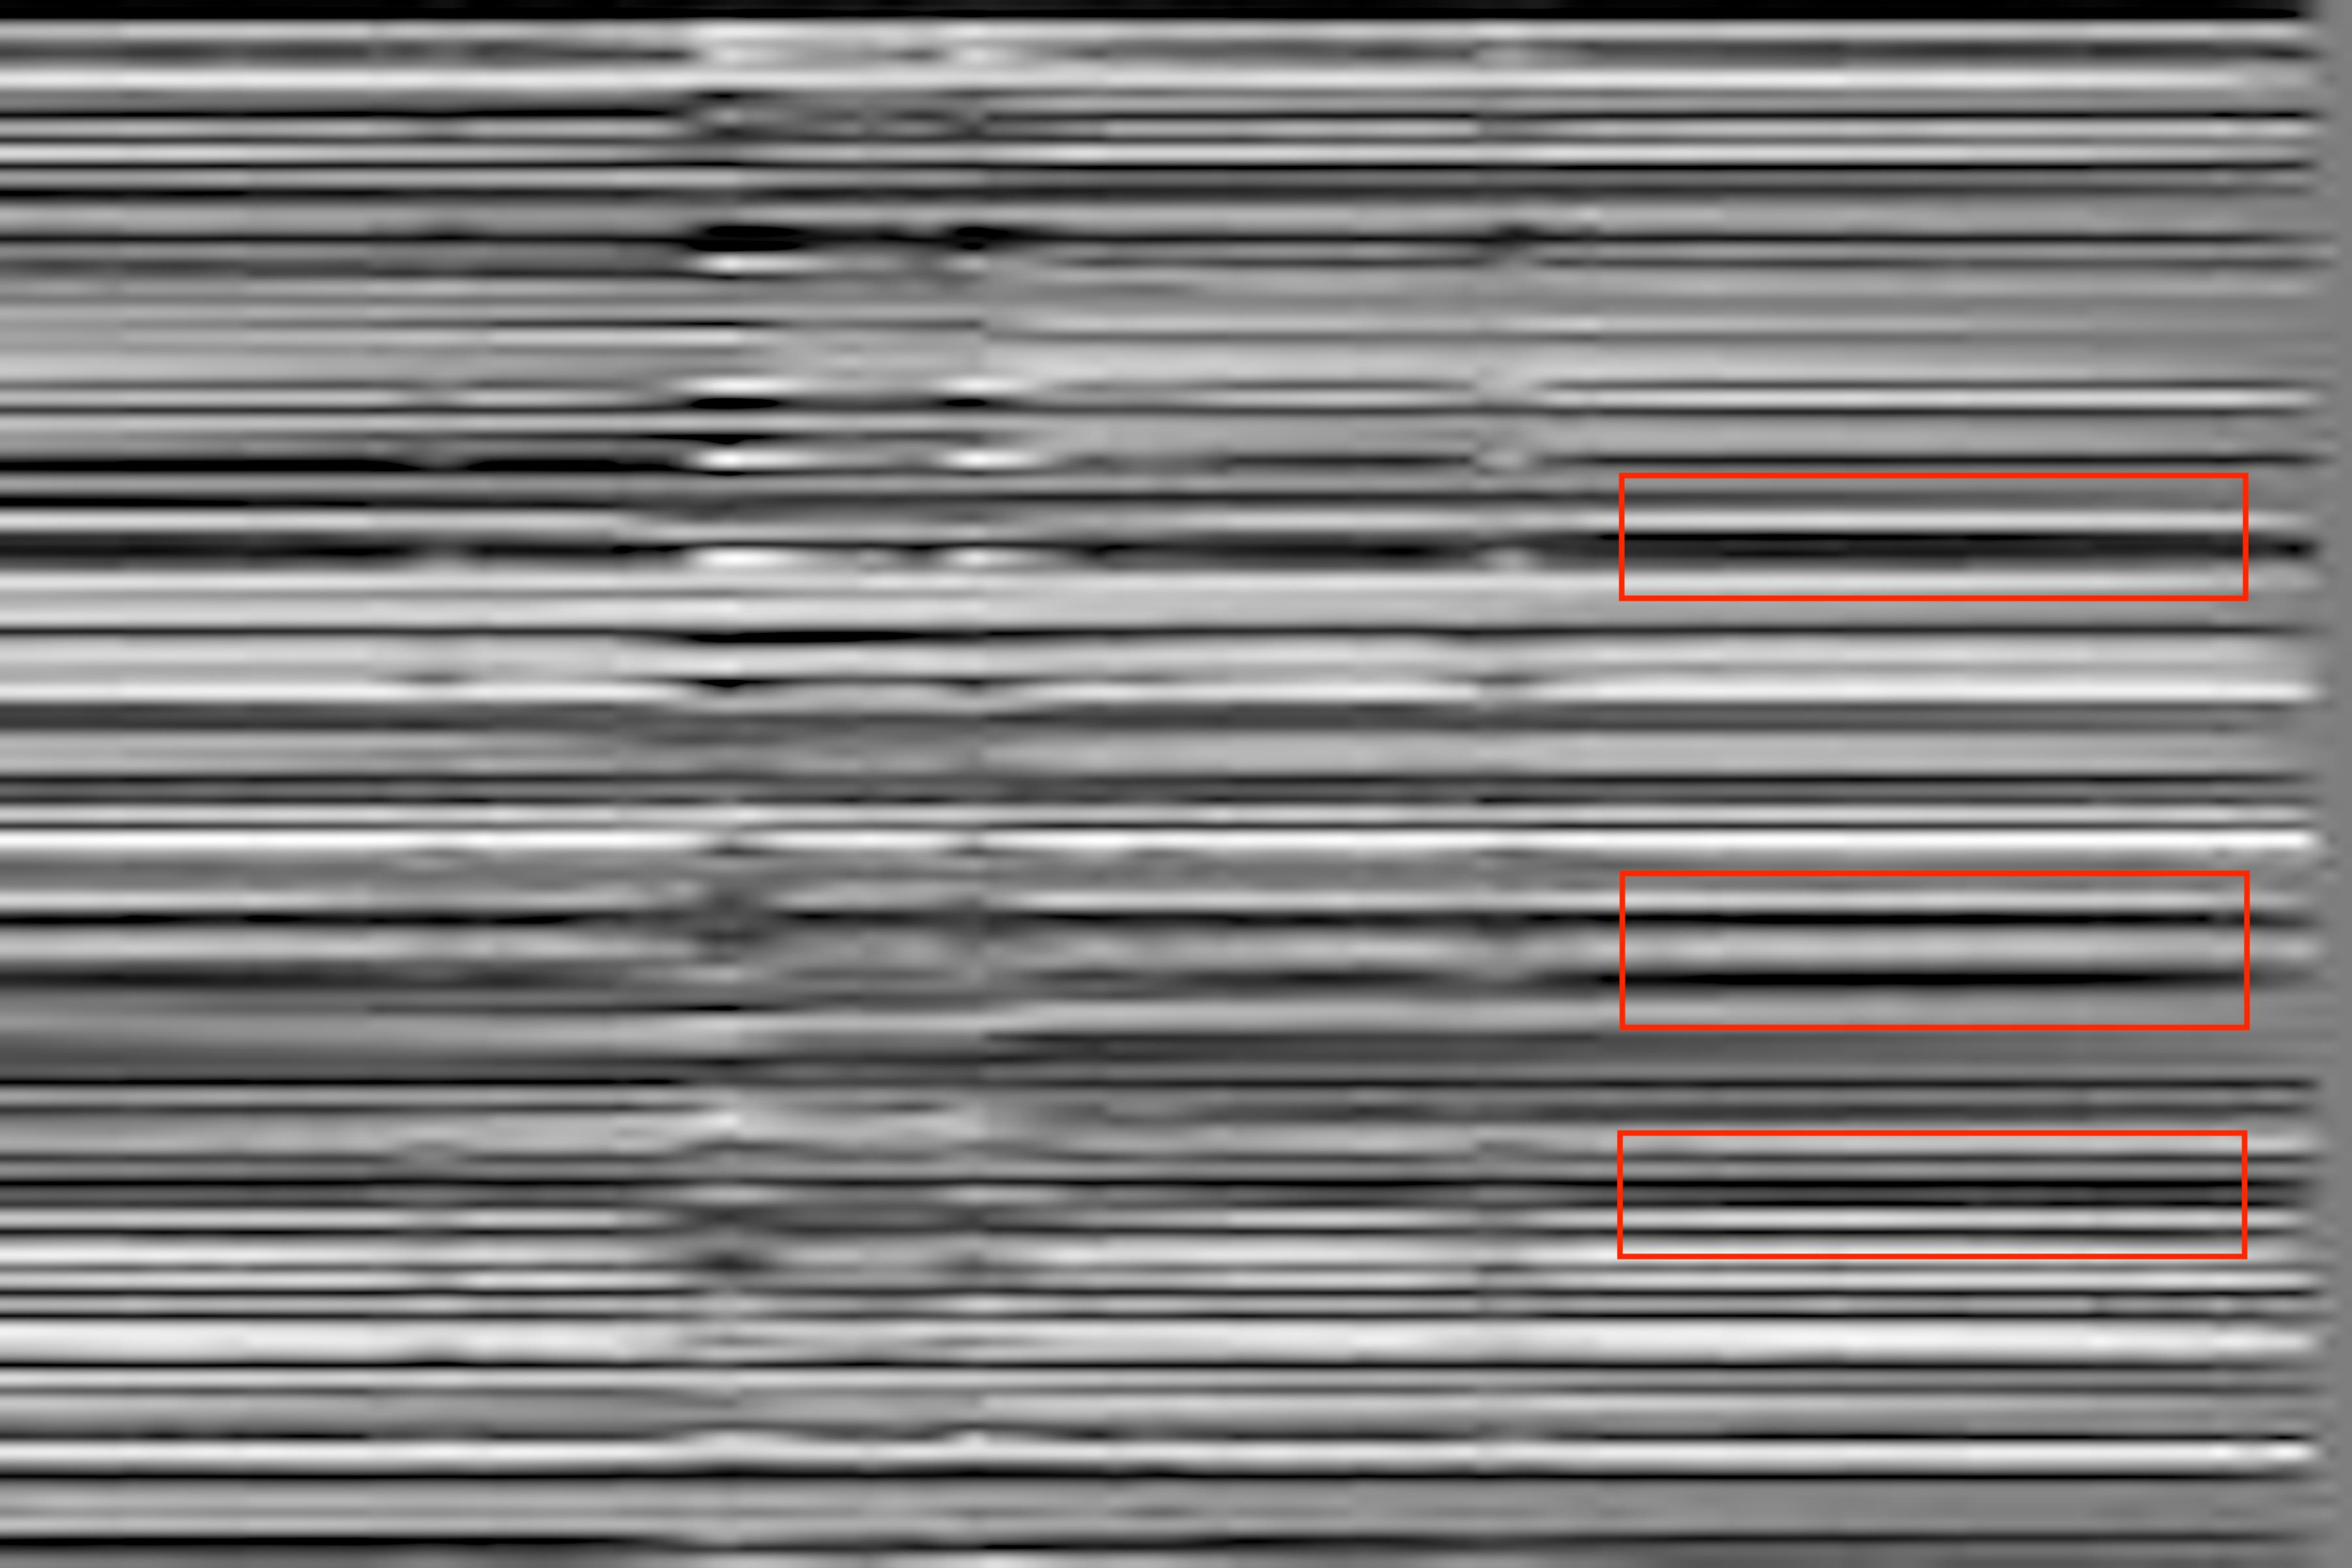
\includegraphics[width=2.7cm]{rnn_out_var_sad}}
    %  \vspace{1.5cm}
    \end{minipage}
    %
    % \setlength{\abovecaptionskip}{0cm}
    % \setlength{\belowcaptionskip}{0cm}
    \caption{Specific active nodes for different emotions (Left: Angry; Middle: Happy; Right: Sad)}
    \label{fig:rnn_emo}
\end{figure}

    
\section{Conclusion}
\label{sec:conclusion}

In this paper, we propose a variable-length neutral network that operates on the spectrogram, to perform emotion classification task from variable-length speech segments. Through inputting the whole sentence into the model, our method can effectively alleviate the confusion between Neutral and other emotions introduced in the traditional fixed-length method in splitting the sentence into smaller fixed-length segments. The weighed accuracies (WA) and the unweighted accuracy (UA) achieves beyond the state of the art accuracy on the common benchmarking dataset IEMOCAP, comparing with the previous work of fixed-length neural network. In the future, we will continue to explore how to use other deep neutral network structure to handle variable-length speech emotion recognition.

%\section{Acknowledgement}
%\label{sec:acknowledgement}
%
%This work is supported by National High Technology Research and Development Program of China (2015AA016305), National Natural Science Foundation of China (NSFC) (61375027, 61433018, 61370023 and 61171116), joint fund of NSFC-RGC (Research Grant Council of Hong Kong) (61531166002, N CUHK404/15) and Major Program for National Social Science Foundation of China (13\&ZD189).


\bibliographystyle{IEEEtran}

\bibliography{refs}


\end{document}
